\documentclass{utart}

\usepackage{plantuml}
\usepackage{float}
\usepackage{graphicx}
\utUseMinted

\title{系统升级工具项目概要设计说明书}
\author{林欣}

\setUTClassify{B级商密}

% 设置文档编号
\setUTIndex{XTSJGJ20221014T_SYS07}

% 设置拟制人信息
\setUTFiction{林欣}{2022-07-18}

% 设置审核人信息
\setUTReview{闫博文}{2022-07-18}

% 设置批准人信息
\setUTApprove{闫博文}{2022-07-18}

% 设置版本号
\setUTVersion{V1.0}

\begin{document}

% 生成封面
\utMakeTitle{}{1.0.0}{2022-07-18}

% 生成修订记录
\utMakeChangeLog{%
    1.0.0 &      创建   &    林欣   &   2022-07-18      \\

    1.0.1 &      根据概要设计评审修改概要设计文档,修改了备份当前系统的时机   &    林欣   &   2022-09-16      \\
    \hline
}

\graphicspath{ {./images/} }

% 生成目录
\utMakeTOC

\newpage

\section{概述}
\subsection{目的}
本文档是基于系统升级工具项目相关需求给出的概要设计文档。在本文档中将给出系统的设计原则、关键结构设计、关键动态流程设计、数据结构设计、非功能性设计、系统部署和实施设计等。

本文总体上将结合形式化设计的方法与文字描述,给出半形式化的概要设计与低层设计,与需求内容相对应,以保证系统设计的严谨性与可实现性。在形式化部分,本文档将主要采取 UML 语言的包图、类图、序列图等进行系统设计。

本文档的适用读者为系统升级工具项目的产品经理、设计人员、开发人员、测试人员以及后续维护人员。

\subsection{术语说明}
\begin{itemize}
    \item LVM: 是一种对磁盘分区进行管理的机制,利用此机制可以实现用户完成分区后,仍然可以改变分区大小。
    \item Atomic-Upgrade: 原子更新是一款通过 OStree 实现系统版本管理的程序,主要功能包括系统备份和系统版本切换。
    \item Deepin-Boot-Kit: 是一套 Grub 管理框架,使用其框架的所有工具需要遵循其规则。
    \item Chroot: 在Unix和类Unix系统上改变程序运行时参考的根目录位置。
    \item dpkg-repack: 可以不依赖于Debian文件夹,从已经安装到系统的应用中生成 deb 包文件
\end{itemize}

\subsection{参考资料}
\begin{enumerate}
    \item https://wiki.debian.org/initramfs
    \item https://ostreedev.github.io/ostree/README-historical
    \item https://access.redhat.com/documentation
\end{enumerate}

\section{系统设计}
\subsection{设计原则}
系统升级工具的目标是给用户提供友好、可靠、便捷、安全的系统升级软件,帮助用户将系统从 V20 升级到 V23,确保用户系统和数据不被破坏,原系统数据和应用在符合 V23 兼容条件下,能正常使用。
\begin{itemize}
    \item 确保升级后,能正常进入 V23 系统桌面并使用系统。
    \item 确保升级失败后能正常回滚到旧系统,并且系统和用户数据不会被篡改或销毁。
    \item 升级程序应采用结构化设计为整体结构设计风格,其中功能模块主要采用面向对象的方法进行设计。
    \item 功能模块之间应避免相互调用,降低模块耦合度。
    \item 模块应遵循最小化职责原则。
    \item 升级过程中应实现失败处理逻辑,尽可能降低对现有系统的影响。
    \item 应遵守 deepin 编码规范。
    \item 升级过程中断,用户可重新进行升级。
\end{itemize}
% 结构设计,面向对象
\subsection{子系统结构}
\subsubsection{结构设计}
UOS 升级工具采用前后端分离的架构设计,整体结构分为升级管理工具和升级工具后端服务两部分,升级管理工具主要负责与用户进行界面交互,升级工具后端服务主要为升级管理工具提供接口服务。
升级工具向镜像服务器获取镜像后,进行新镜像根目录重构建后,调用原子更新提供的接口实现系统的备份和升级,在系统升级成功后,将 V20 系统上安装的部分应用,迁移到 V23 系统中。
升级工具与更新平台建立连接上报埋点数据并调用更新平台接口来判断是否进行批量自动化升级。各个组件之间的关系如图 2.1 所示:
% 面向对象,也就是将功能模块化。 
\begin{figure}[H]
    \centering
    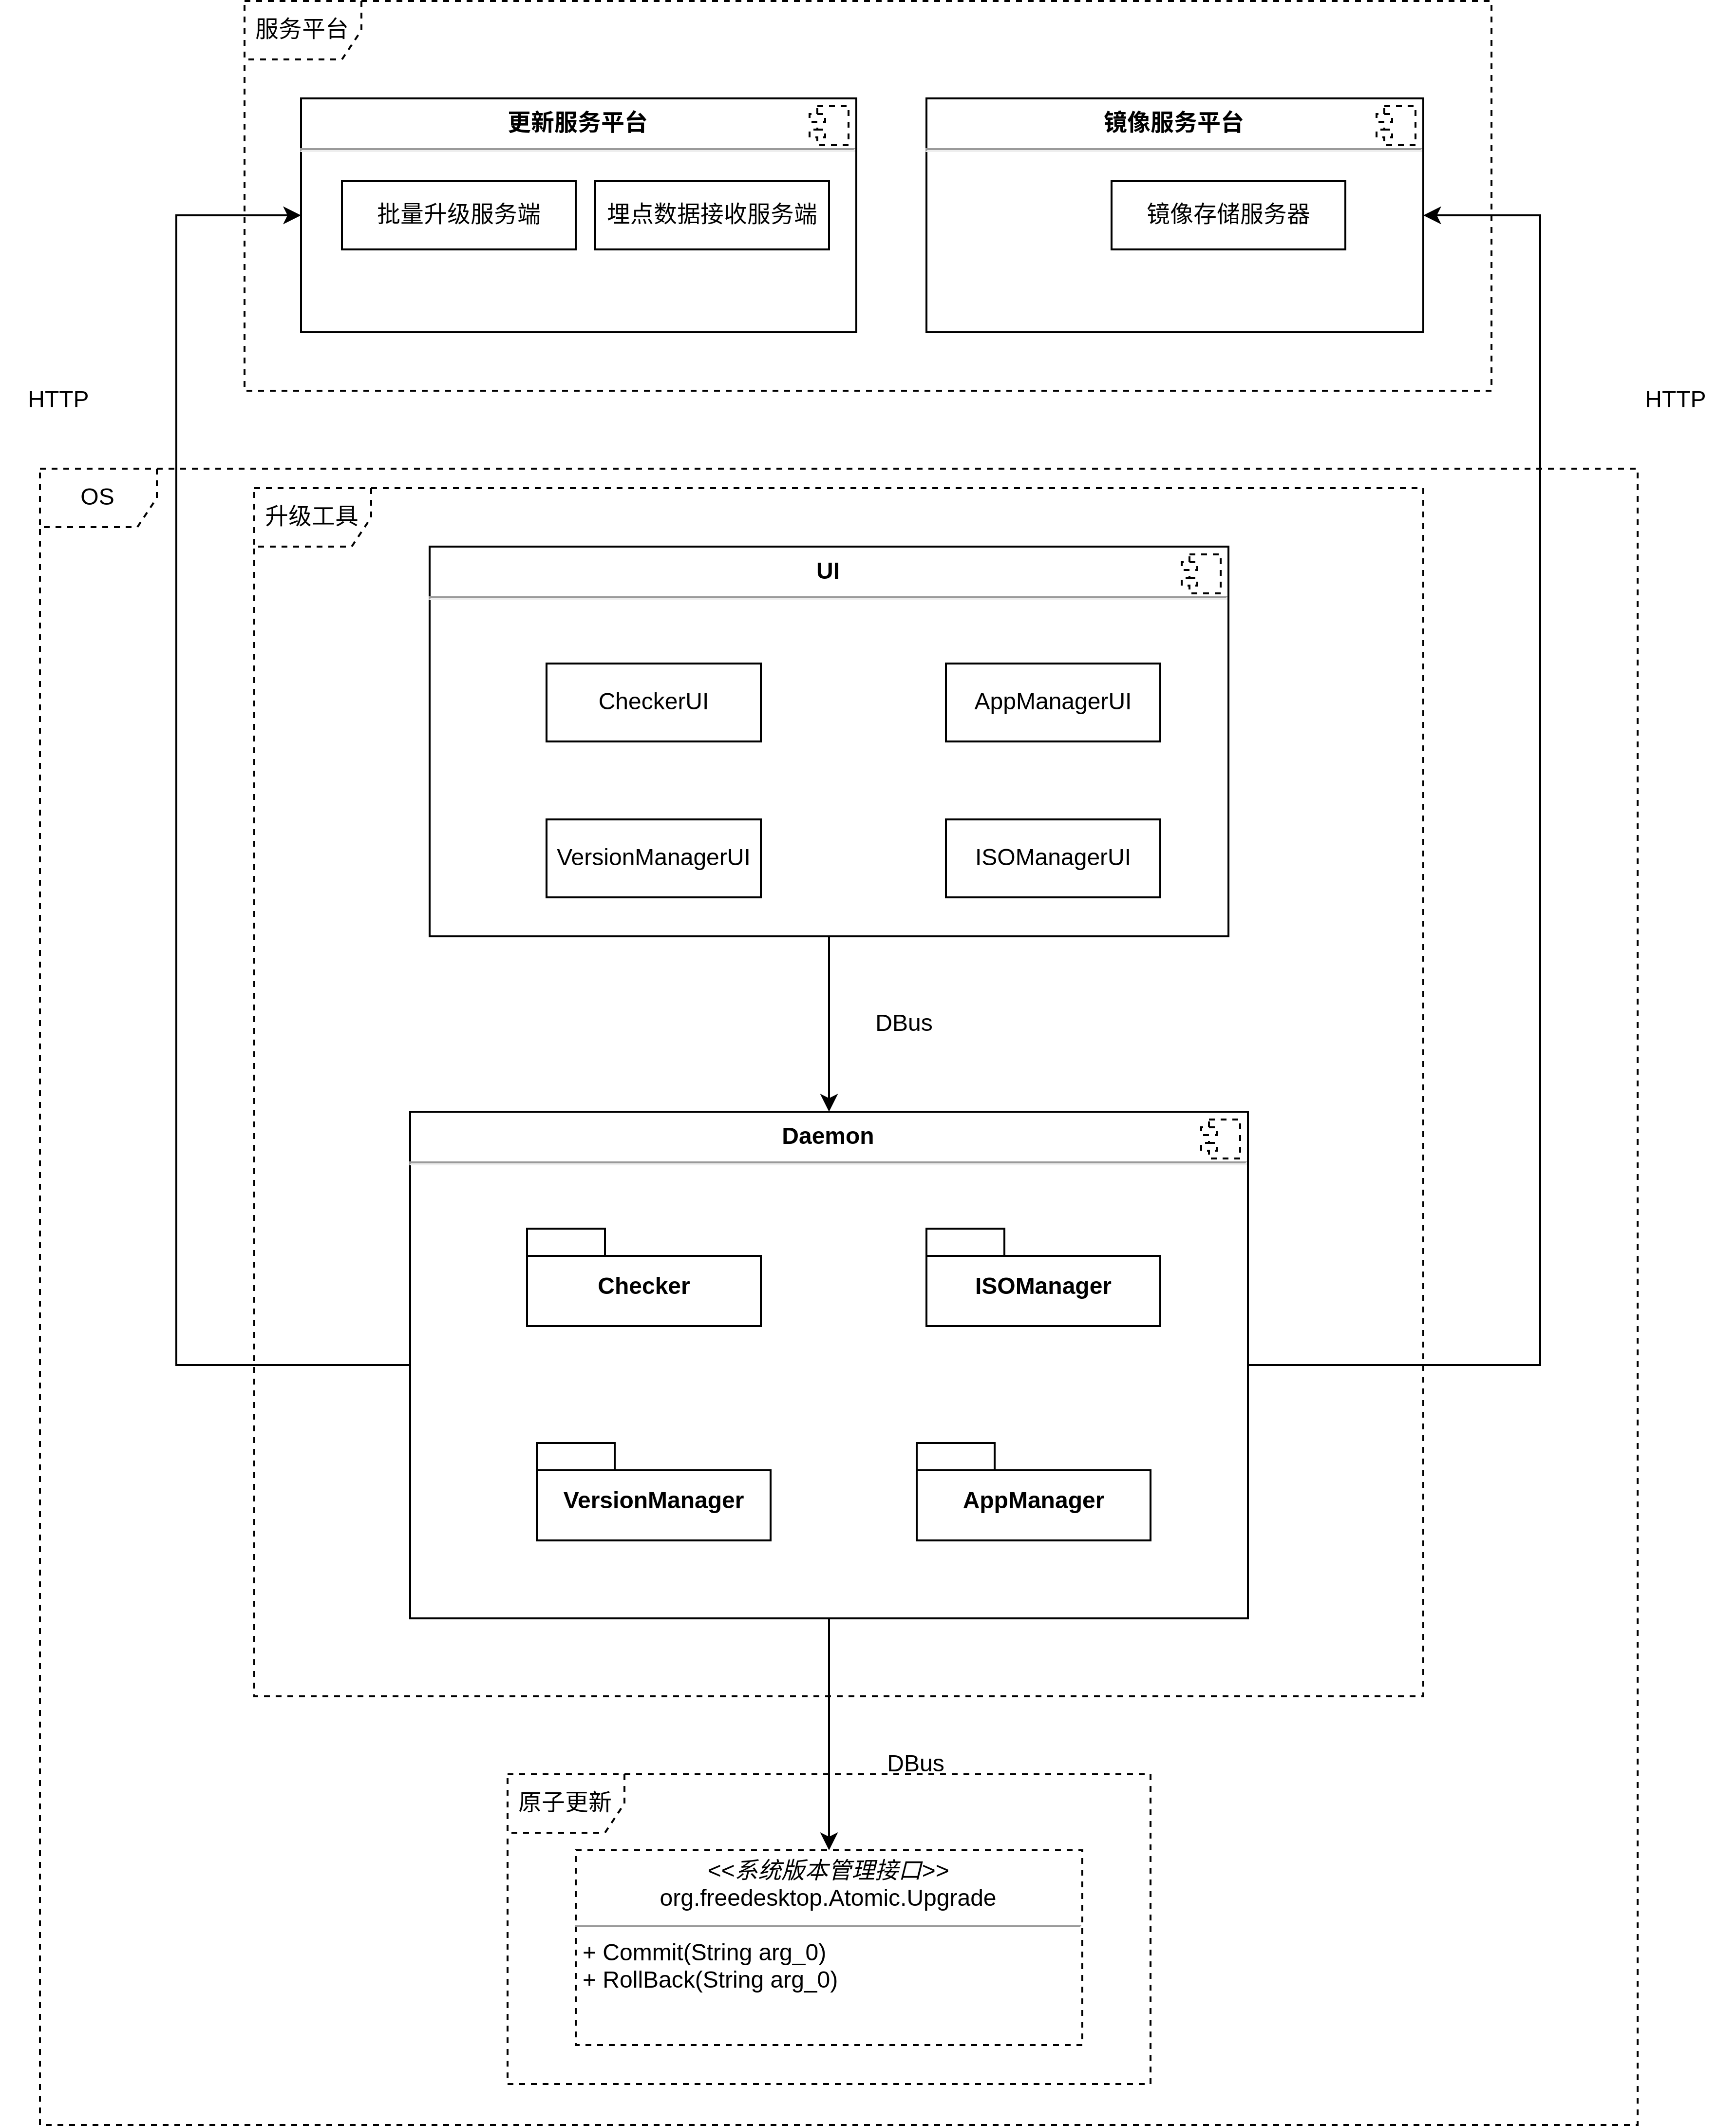
\includegraphics[width=\textwidth]{main}
    \caption{升级工具结构图}
    \label{fig:upgradestruct}
\end{figure}
% 抽象的公共组件
% 层次结构 
% 前端对象之间的交互
% 自顶向下逐层分解 
% 以核心对象为粒度
% 混合面向过程,面向对象,分层设计相
% 标明模块之间通讯方式
% 应用迁移如何对包进行分类,以及分类后的处理。

\paragraph{升级管理工具}
升级管理工具为升级工具前端页面,主要职责是面向用户,提供升级流程控制以及升级状态显示等功能,选用 C++ 作为主要开发语言,使用 QT 和 DTK 等开发库完成界面开发。
升级管理工具不需要关心主要功能的底层实现,功能模块的实现由升级工具后端服务实现并提供接口,升级管理工具主要需要关注界面的开发以及业务逻辑的交互。主要功能如下:
\begin{itemize}
    \item 检查用户环境是否满足升级条件, 包括系统版本检查、CPU 架构检查、系统激活状态和存储剩余空间等。
    \item 检查旧系统过渡到新系统软件变更状态,包括软件的新增减少以及兼容性。
    \item 获取 V23 镜像文件并进行校验。
    \item 启动升级前的系统备份、升级前新系统根目录的重构建、提交以及系统升级。
    \item 显示系统升级后的状态。如成功或失败。
    \item 系统升级成功后,启动应用迁移流程。
    \item 配合升级工具后端服务完成内网批量升级。
\end{itemize}
结构设计如图 2.2 所示:
\begin{figure}[H]
    \centering
    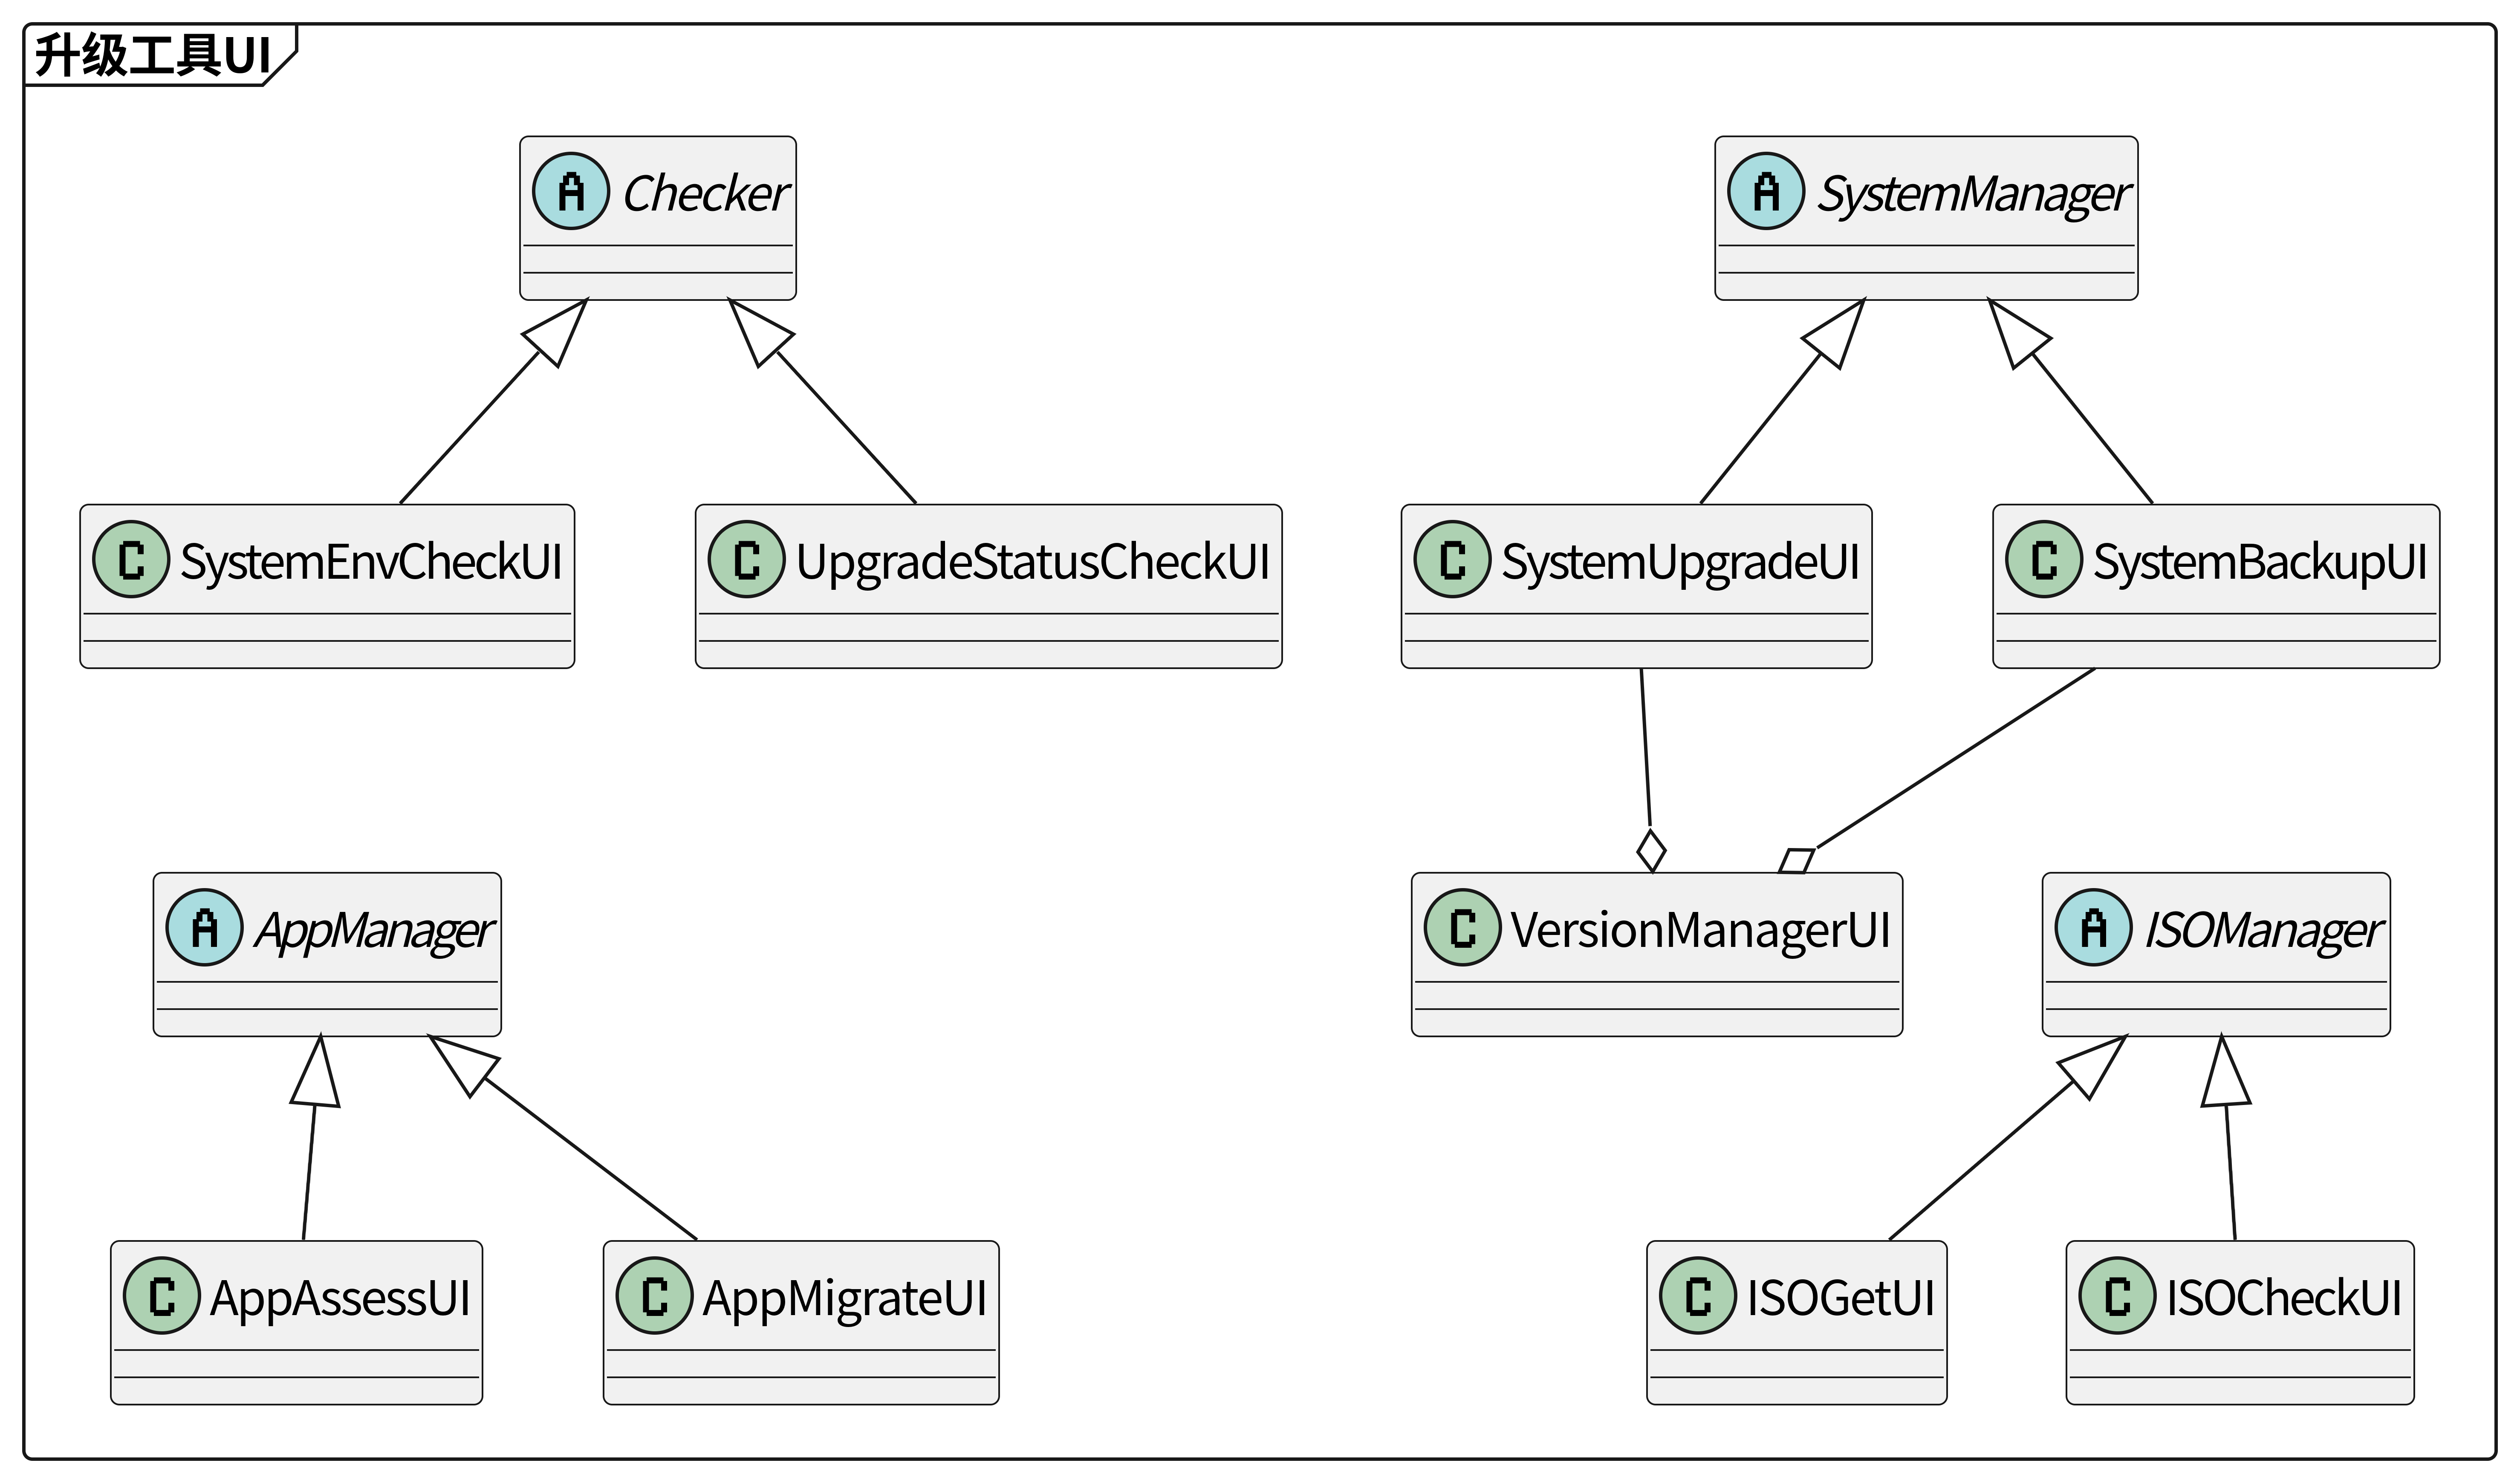
\includegraphics[width=\textwidth]{toolstruct}
    \caption{升级管理工具结构图}
    \label{fig:toolstruct}
\end{figure}

% 主要包括镜像获取、镜像根目录重建、系统备份、系统升级、批量升级以及数据埋点等功能。
\paragraph{升级工具后端服务}
升级工具后端服务主要选用 GO 语言实现,作为升级管理工具的后端,主要职责是完成功能接口的组装和实现,通过 DBus 提供给升级管理工具。
升级工具后端服务通过依赖原子更新接口实现系统的备份和更新,通过依赖外部服务平台实现 V23 镜像的获取以及批量升级指令信息。主要功能如下:
\begin{itemize}
    \item 实现系统更新条件检查接口。
    \item 实现系统升级完成后状态检查接口。
    \item 实现 V23 镜像获取与校验接口。
    \item 根据 V23 镜像文件重新构建用于替换原系统目录的系统根目录。
    \item 通过原子更新系统的接口来封装系统备份与更新接口。
    \item 实现软件评估接口,用于比较新旧系统之间软件差异,以及软件被迁移后在新系统上的兼容性。
    \item 通过调用更新平台服务端接口获取内网批量升级指令信息,根据指令信息判断是否需要进行自动化批量升级。
    \item 收集用户系统信息以及升级状态信息并发送给更新平台。
\end{itemize}

结构设计如图 2.3 所示:
\begin{figure}[H]
    \centering
    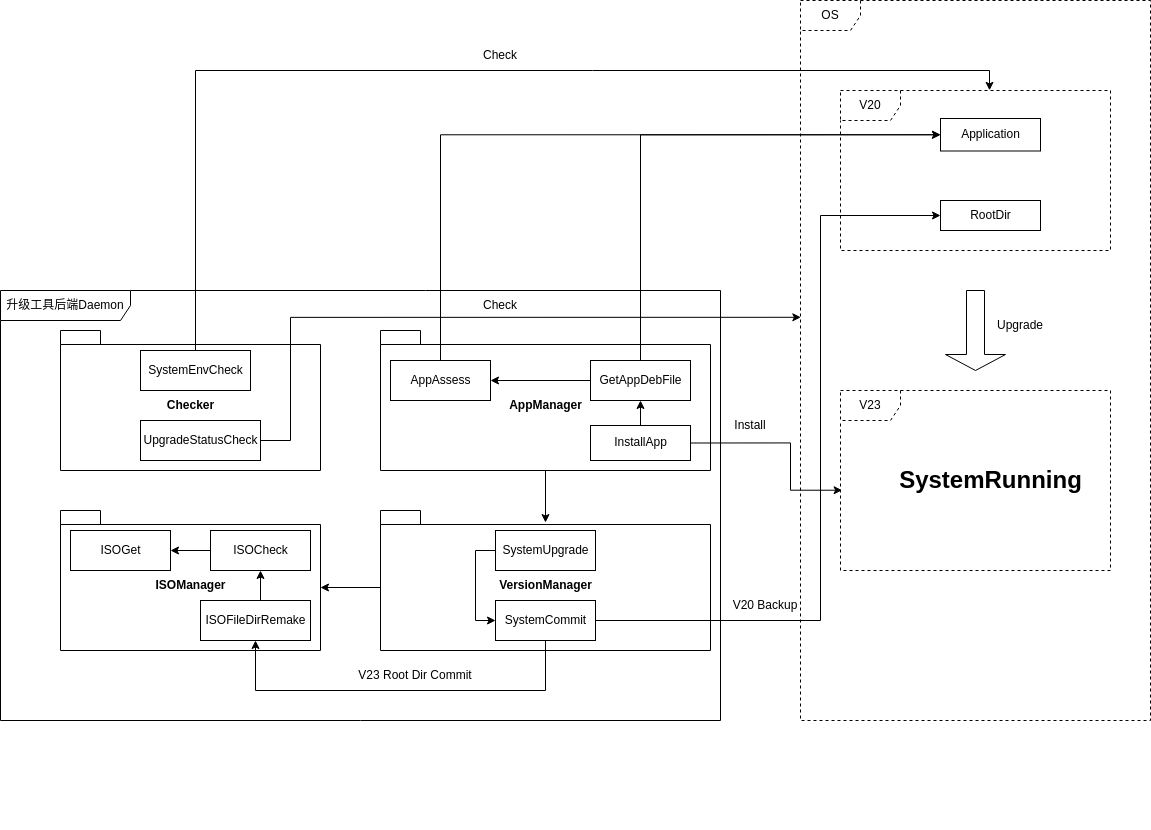
\includegraphics[width=\textwidth]{daemon}
    \caption{后端服务结构图}
    \label{fig:daemon}
\end{figure}

\subsubsection{外部依赖组件描述}

\paragraph{更新平台服务}
更新平台的主要职责是系统更新管理。主要功能如下:
\begin{itemize}
    \item 提供批量升级管理接口,用于告知调用方当前用户系统是否需要进行自动化批量升级。
    \item 接收UOS升级工具上报的埋点数据,主要记录用户升级过程中的相关信息,如系统相关信息,升级是否成功等。
\end{itemize}

\paragraph{原子更新}
原子更新为系统底层公共库,对外提供接口进行系统版本管理,主要功能如下:
\begin{itemize}
    \item 提供系统备份接口,将系统备份快照保存在本地仓库。
    \item 生成系统备份版本对应的 Grub 引导选项。
    \item 提供系统回滚接口,将系统版本切换到到指定的备份版本上。
\end{itemize}

\paragraph{引导管理}
升级工具在系统升级过程中涉及到的引导管理和系统根目录替换逻辑的调用是通过原子更新 Atomic-Manager 程序接口进行管理。

\subsection{关键流程设计}
\subsubsection{升级工具主流程设计}
升级工具主流程由升级管理工具、升级工具后端服务、原子更新和外部服务平台等组件共同完成,主流程图如图2.4所示:
\begin{figure}[H]
    \centering
    \begin{plantuml}
        @startuml
            start
            :启动升级工具检查系统环境;
            while (用户当前系统环境是否满足升级条件) is (否)
            :展示环境检查失败原因;
            if (用户是否重新检查) then (是)
            :重新检查;
            else (否)
            :退出升级工具;
            stop
            endif
            endwhile(是)
            :备份当前系统;
            :准备系统升级环境;
            :重启开始系统升级;
            if (系统是否升级成功) then (是)
            :迁移原系统应用;
            else (否)
            :回滚到原系统;
            endif
            stop
        @enduml
    \end{plantuml}
    \caption{升级工具主流程图}
    \label{fig:main}
\end{figure}

当前系统的软硬件环境需要满足的条件包括:
\begin{itemize}
    \item 系统版本为1060专业版或1060社区版。
    \item 系统激活状态为已激活。
    \item CPU 架构为 X86 或 ARM。
    \item 存储剩余空间大于备份和升级所需的空间。
    \item 电源和网络为已连接状态。
\end{itemize}

\subsubsection{升级工具系统检查模块流程设计}
系统检查模块主要包括系统升级条件检查以及软件检查,实现流程如图2.5 所示:
\begin{figure}[H]
    \centering
    \begin{plantuml}
        @startuml
        actor 用户 as A 
        box "UOS 升级工具" #lightblue
        participant "deepin-system-upgrade-tool" as UT
        participant "deepin-system-upgrade-daemon" as UD                             
        endbox
        box "V20运行时系统" #lightblue
        participant "running-system" as S
        endbox
        A -> UT: 启动升级管理工具
        UT -> UT: 初始化 CheckerUI 中升级前系统检查模块
        UT -> UD: 调用 Checker 接口检查系统环境
        UD -> S: 检查系统状态
        S -> UD: 返回状态信息
        UD -> UT: 返回 Check 结果  
        alt 不满足条件
        loop
        UT -> UT: 等待用户触发退出或重新检查
        end
        else 满足条件
        UT -> UT: 初始化AppManagerUI 中软件检查模块
        UT -> UD: 调用 AppManager 接口 Assess 函数进行软件评估
        UD -> UT: 返回软件检查结果
        @enduml
    \end{plantuml}
    \caption{系统检查时序图}
    \label{fig:systemcheck}
\end{figure}

\subsubsection{升级工具升级准备模块流程设计}
升级工具系统准备模块主要包括系统备份以及 V23 根目录重构建并提交等功能,实现流程如图2.6所示:
\begin{figure}[H]
    \centering
    \begin{plantuml}
        @startuml
        actor 用户 as A 
        box "UOS 升级工具" #lightblue
        participant "deepin-system-upgrade-tool" as UT
        participant "deepin-system-upgrade-daemon" as UD                             
        endbox

        box "系统服务" #lightblue 
        participant "atomic-upgrade" as AU
        endbox
        
        box "外部服务" #lightblue
        participant "iso-server" as IS
        endbox

        box "V20运行时系统" #lightblue
        participant "running-system" as S
        endbox

        A -> UT: 环境检查通过,进入升级准备阶段
        UT -> UT: 初始化 VersionManagerUI 中升级准备模块
        UT -> UD: 调用 ISOManager 接口中 Get 函数获取镜像
        UD -> IS: 利用 wget 下载镜像文件
        UT -> UD: 调用 ISOManager 接口中 Check 函数检查镜像
        UT -> UD: 调用 VersionManager 接口中 PrepareForUpgrade 函数
        
        UD -> S: 挂载镜像文件到指定目录
        UD -> S: 将镜像根目录文件拷贝到 rootfs 目录
        UD -> S: chroot 到 rootfs 目录进行新镜像根目录重构建
        UD -> S: 将新系统根目录下的/etc 目录合并到当前系统对应目录中
        UD -> AU: 调用 Commit 接口提交 V23 镜像文件夹中指定的系统目录
        UT -> UT: 初始化 VersionManagerUI 中系统备份模块
        UT -> UD: 调用 VersionManager 接口中 BackupSystem 函数
        UD -> AU: 调用 Commit 接口备份当前系统
        UD -> S: 修改系统 Grub 为默认引导 V23 引导分支

        @enduml
    \end{plantuml}
    \caption{升级准备时序图}
    \label{fig:prepareupgrade}
\end{figure}

Commit 提交的系统目录主要有/usr、/boot 和/var 目录,以上目录足以满足系统升级的需求。
为防止升级过程导致/etc 目录下被修改或新添加文件被覆盖或丢失,所以选择保留/etc 目录,并且将新系统根目录下的/etc 目录合并到当前系统对应目录中,合并的原则是文件存在即跳过,不存在则拷贝,但是有些文件与新系统强耦合,需要强行覆盖,主要有以下几类:
\begin{enumerate}
    \item 版本配置:系统版本配置信息,如/etc/os-version,/etc/os-release。
    \item 认证配置:PAM 模块配置文件,如/etc/pam.d 文件夹。
\end{enumerate}


其中原子更新工作原理如下:
\begin{itemize}
    \item 利用 OStree 快照功能,生成当前系统文件快照保存在本地。
    \item 每次保存快照会生成对应的 Grub 选项。
    \item 选中 Grub 选项后,原子更新程序会查询并使用对应的系统快照版本文件来替换系统根目录,完成系统版本切换。
\end{itemize}

\subsubsection{V23系统根目录重构建流程设计}
从镜像文件解压出的根目录文件无法满足系统的运行要求,直接替换会导致系统无法启动等问题。因此需要chroot到新的镜像文件根目录下,执行 deb 包的安装、用户数据迁移以及 Grub 更新等操作对新镜像根目录进行改造。
主要流程如图2.7 所示:

\begin{figure}[H]
    \centering
    \begin{plantuml}
        @startuml
        start
        :挂载镜像文件到/medio/iso 目录;
        :将 squashfs 文件挂载到/medio/iso/squashfs 目录中;
        :将 squashfs 目录中的根文件夹拷贝到/medio/iso/rootfs 目录中;
        :将当前系统根目录下需要迁移的文件拷贝到 rootfs 下对应的目录中;
        :挂载当前系统运行依赖目录到 rootfs 中对应目录上;
        :chroot 到 rootfs 目录;
        :在新环境下加装新的软件包如 grub;
        :执行 grub-install 安装 grub;
        :执行 update-grub 更新 grub.cfg;
        :退出 chroot 环境;
        :V23 系统目录准备完成;
        end
        @enduml
    \end{plantuml}
    \caption{根目录准备流程图}
    \label{fig:rootmake}
\end{figure}

\subsubsection{升级工具系统升级模块流程设计}
系统升级模块主要描述系统升级过程,实现流程图如图2.8所示:
\begin{figure}[H]
    \centering
    \begin{plantuml}
        @startuml
        actor 用户 as A 
        box "UOS 升级工具" #lightblue
        participant "deepin-system-upgrade-tool" as UT
        participant "deepin-system-upgrade-daemon" as UD                             
        endbox

        box "V20运行时系统" #lightblue
        participant "running-system" as S
        endbox

        box "系统服务" #lightblue 
        participant "atomic-upgrade" as AU
        endbox

        A -> UT: 升级准备完成,现在开始升级
        UT -> UT: 初始化 VersionManagerUI 中启动升级模块
        UT -> UD: 调用 VersionManager 接口中 StartSystemUpgrade 函数
        UD -> S: 重启系统
        S -> S: 进入 initrd 阶段
        S -> AU: 调用原子更新 RollBack 接口执行系统版本切换
        UT -> UT: 初始化 CheckerUI 中升级后系统检查模块
        UT -> UD: 调用 Checker 接口中 Checker 函数
        UD -> S: 检查升级后的系统状态
        S -> UD: 返回状态信息
        UD -> UT: 返回检查结果
        UT -> UT: 显示检查结果
        alt 成功
        UD -> AU: 删除
        UT -> UT: 初始化 CheckerUI 中升级后系统检查模块
        UT -> UD: 调用 Checker 接口中 PostCheck 函数
        UD -> S: 检查系统状态
        S -> UD: 返回状态信息
        UD -> UT: 返回检查结果
        UT -> UT: 显示检查结果
        UT -> UT: 初始化AppManagerUI 中应用迁移模块
        UT -> UD: 调用AppManager 接口中 AppMigrate 函数
        UD -> UT: 发送应用迁移进度信息
        UT -> UT: 显示界面动画展示迁移进度
        UD -> UT: 迁移完成
        else 升级失败
        AU -> S: 回滚到原系统
        end
        @enduml
    \end{plantuml}
    \caption{升级流程时序图}
    \label{fig:upgrade}
\end{figure}

\subsubsection{升级工具批量升级模块流程设计}
批量升级功能主要用于满足内网企业用户进行大规模自动化系统升级需求,预装升级工具的内网用户,会自动检测当前系统环境是否满足自动化升级的条件,如满足,用户无需额外操作,
升级过程会全程自动化执行。实现流程如图2.9所示:
\begin{figure}[H]
    \centering
    \begin{plantuml}
        @startuml
        actor 用户 as A 
        box "UOS 升级工具" #lightblue
        participant "deepin-system-upgrade-tool" as UT
        participant "deepin-system-upgrade-daemon" as UD                             
        endbox

        box "V20运行时系统" #lightblue
        participant "running-system" as S
        endbox
        
        box "外部服务" #lightblue
        participant "upgrade-platform-server" as UPS
        endbox

        A -> S: 启动办公系统
        S -> UD: 升级工具后台服务自启动
        UD -> UPS: 连接更新平台服务端
        UD -> UPS: 调用更新平台接口检查当前用户是否满足批量自动化升级条件
        UPS -> UD: 返回检查结果
        UD -> UD: 解析检查结果
        alt 需要升级
        UD -> UT: 启动升级管理工具
        UT -> UT: 执行自动化升级流程
        else 不需要升级
        UD -> UD: 进程终止
        end        
        @enduml
    \end{plantuml}
    \caption{批量升级时序图}
    \label{fig:mulkupgrade}
\end{figure}

\subsubsection{应用迁移流程设计}
应用迁移主要针对在旧系统上已安装但在V23系统上未安装的应用。详细流程如图2.10所示:

% 应用迁移会出现依赖风险。
\begin{figure}[H]
    \centering
    \begin{plantuml}
        @startuml
        box "UOS 升级工具" #lightblue
        participant "deepin-system-upgrade-daemon" as UD                             
        endbox

        box "V23运行时系统" #lightblue
        participant "v23-system" as NS
        endbox
        
        box "外部服务" #lightblue
        participant "iso-server" as IS
        participant "deb-repository" as DR
        endbox

        box "V20系统" #lightblue
        participant "v20-system" as OS
        endbox

        UD -> IS: 获取镜像仓库中新镜像应用预装信息的文件
        UD -> OS: 解析旧系统 /var/lib/dpkg/status 文件获取当前系统安装的应用列表
        UD -> UD: 比较文件差异获取 deb 包变更详细信息
        loop
        alt 需要迁移的应用包存在于当前系统仓库
        UD -> DR: 下载应用 deb 包
        else 不存在于当前的系统仓库
        UD -> NS: 将 ostree 仓库中的旧系统快照 checkout 到指定目录
        UD -> OS: chroot 到旧系统目录提取应用 deb 包文件(包括无法从当前仓库获取的依赖包)
        UD -> OS: 使用 dpkg-repack 工具重新生成 deb 包
        UD -> OS: 退出 chroot 环境
        end
        UD -> NS: 使用 apt 工具模拟 deb 包的安装
        alt deb 包安装模拟通过 
        UD -> NS: 将 deb 安装到新系统中
        else 包安装模拟不通过
        UD -> UD: 将应用打上迁移失败标记返回给升级管理工具展示给用户
        end
        end
        @enduml
    \end{plantuml}
    \caption{应用迁移时序图}
    \label{fig:appmig}
\end{figure}

\paragraph{应用包的安装}
系统中安装的应用涉及到多种来源,可以归纳为系统原装应用、源仓库下载应用、自行从网站下载 deb 包进行安装的应用。为了保证系统功能的完整性,应用迁移以 deb 包为单位进行迁移。
应用 deb 包迁移过程中,涉及到 deb 包的获取、deb 包的模拟安装以及 deb 包的正式安装,其中,deb 包的获取主要方式是从仓库下载或使用 dpkg-repack 工具进行生成,deb 包的模拟安装使用 apt 工具配合 -simulate 参数进行模拟安装,模拟安装不会对系统产生任何修改,如果出现依赖关系不满足的情况,apt 命令返回非零常数,deb 包的正式安装依赖于模拟安装的结果。
安装应用前会检查应用 deb 包的依赖信息,如在新系统中依赖包关系不满足,并且新系统仓库中不存在此依赖包,则需要在将依赖包也进行迁移。

\paragraph{应用配置文件处理}
升级工具在升级过程中,保留了大部分原系统的配置文件,那么在软件包安装的过程中,为了避免旧配置文件被覆盖,主要有以下处理方式:
\begin{enumerate}
    \item 部分应用 deb 包内 debian 目录下包含了 conffiles 文件,此文件可以防止应用包在安装过程中对 conffiles 包含的配置文件进行覆盖。这种软件包升级工具在包安装过程中不用考虑配置文件覆盖问题。
    \item 部分应用 deb 包内 debian 目录下没有包含 conffiles 文件,因此在安装软件包是会弹出选项询问用户是否保留旧配置文件,升级工具默认选择“是”来防止配置文件被覆盖。
\end{enumerate}

\subsubsection{问题修复框架设计}
升级工具问题修复框架不执行实际的修复逻辑,主要负责协助应用修复系统升级后出现的应用兼容性问题。工作原理如图2.11所示:

\begin{figure}[H]
    \centering
    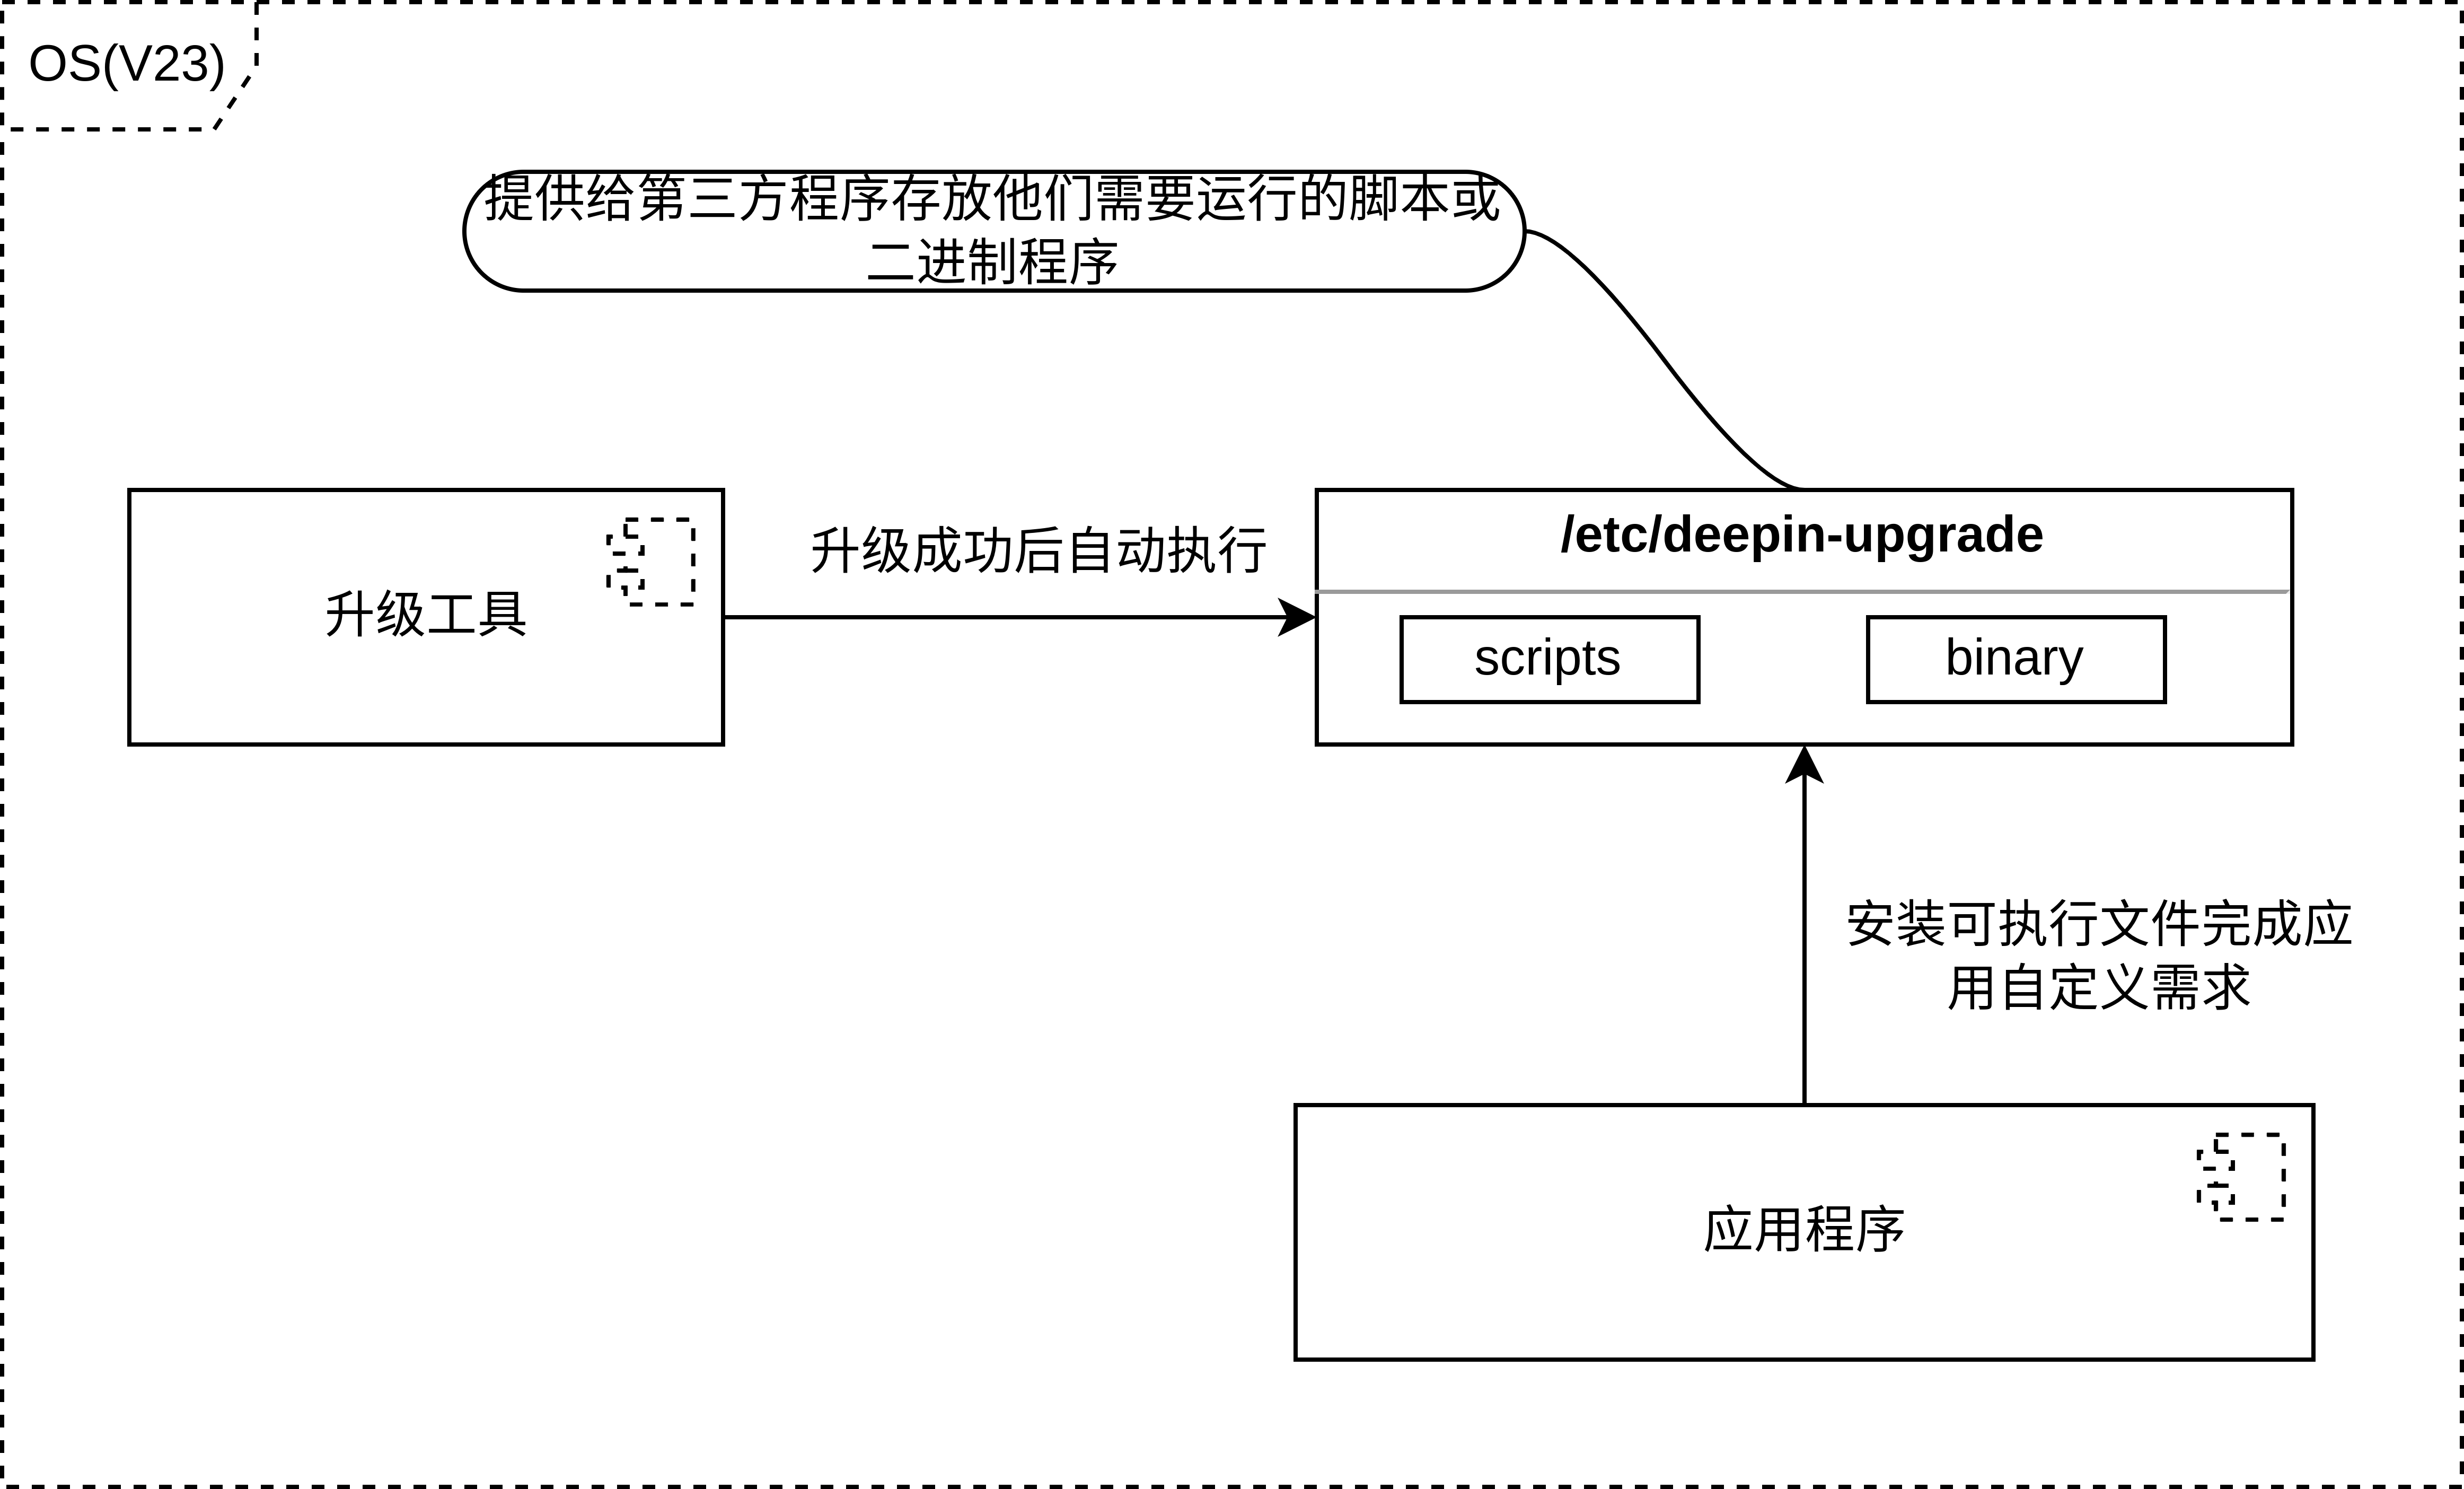
\includegraphics[width=\textwidth]{repaireframe}
    \caption{问题修复框架图}
    \label{fig:repaire}
\end{figure}

执行流程如下:
\begin{enumerate}
    \item 向应用提供一个固定的系统目录。
    \item 应用将升级后执行修复流程的二进制或脚本文件安装到固定目录下。
    \item 升级工具在升级成功后会遍历并自动执行该目录下所有的可执行文件。
\end{enumerate}

\subsubsection{分区合并流程设计}
升级工具提供卷管理功能,若用户使用LVM卷功能对分区进行管理,升级工具可支持分区合并。如用户存在A/B分区,并且使用了卷功能来管理分区,升级工具需要将A/B分区合并。
LVM卷管理原理如下:
\begin{itemize}
    \item 将磁盘分区创建成对应的物理卷Physical Volume*
    \item 将创建的物理卷PV根据自己的需求分成若干卷组Volume Group*
    \item 在各个卷组上根据自己的需求创建指定大小的逻辑卷Logical Volume*
    \item 逻辑卷的功能与磁盘分区相似,进行格式化后可直接挂载到指定目录,优点在于可根据自己的需求调整逻辑卷大小并支持逻辑卷合并,还可实现磁盘的缩减与扩容。
\end{itemize}

升级工具分区合并功能要求分区管理必须基于LVM卷管理功能,否则不支持分区合并,详细流程设计如图2.12所示
\begin{figure}
    \centering
    \begin{plantuml}
        @startuml
        box "升级工具" #lightblue
        participant "deepin-system-upgrade-daemon" as UD
        endbox

        box "系统分区" #lightblue
        participant "Rootb" as RB
        participant "Roota" as RA
        endbox

        UD -> RB: 挂载Rootb分区到指定目录
        UD -> RB: 格式化并卸载Rootb分区
        UD -> RB: 删除Rootb分区对应的逻辑卷
        alt Rootb 和 Roota在同一个逻辑卷组
        UD -> RA: 直接利用Rootb原空间扩容Roota逻辑卷
        else 不在同一个逻辑卷组
        UD -> RB: 将Rootb分区对应的物理卷添加到Roota所在卷组中
        UD -> RA: 利用新添加的Rootb空间扩容Roota逻辑卷
        end
        @enduml
    \end{plantuml}
    \caption{分区合并时序图}
    \label{fig:partition}
\end{figure}

% 类,接口,对象。
\subsection{关键数据结构设计}
% TODO 关键数据结构可以从应用数据迁移,替换目录,应用迁移进行入手,以及V23版本号
% 是否需要应用迁移info.jon(旧系统有,V23系统没有的包),通过比较是否需要缓存,缓存的目的是下次能用到,这个缓存的作用是什么
% 直接对比找出V23系统有旧系统没有的包,然后从仓库下载到指定目录。切换到V23后直接安装对应目录下的所有包

\subsubsection{升级工具配置文件}
升级工具配置文件使用 YAML 文件格式,主要记录升级过程以及应用迁移过程依赖的关键配置信息,此配置文件满足功能性、拓展性以及兼容性,用户或程序可通过修改此配置文件来进行配置文件定制化迁移。文件格式如下:

\begin{minted}{c}
version: # 配置文件版本
tranfer: # 系统升级控制
 min_version: # 最小版本要求
 distro: "v20"
 subversion: "1060"
 integrity: true # 是否进行完整性检查
source:
 url: "https://xxx" # 数据源地址
 type: "http" # 源数据获取方式
 target:
 sys_dirs: # 需要进行替换的系统目录
  - "/boot"
  - "/usr"
  - "/var"
backup_apps: true # 是否备份应用
migrate: # 文件迁移
-
 label: "config" # 文件功能类别
 type: "file" # 文件属性
 direction: "V23" # 文件迁移方向,用 V20 系统文件替换对应的 V23 系统文件
 targets:
  - "/usr/lib/dpkg-db" #针对/usr、/boot 和/var 目录
  - "/var/spool"
-
 label: "pam"
 type: "file"
 direction: "V20" # 文件迁移方向,用 V23 系统文件替换对应的 V20 系统文件
 targets:
  - "/etc/pam.d" # 针对升级过程中不进行替换的目录
  - "/etc/os-version"
  - "/etc/os-release"
\end{minted}

\subsection{主要人机交互设计}
人机交互设计原型图见《产品原型设计图》。

\section{非功能性设计}
\subsection{安全性}
安全性设计主要从数据安全性、系统安全性等方向进行设计,详细描述如下:

\paragraph{系统安全性}
\begin{enumerate}
    \item 升级工具后端会对调用程序进行身份认证,只接受升级管理工具的调用,从而保证系统不会被恶意接口调用导致出现异常。
    \item 升级工具会对调用者进行身份验证,需要有管理员权限才能允许升级。
\end{enumerate}

\paragraph{数据安全性}
数据安全性主要包括系统根目录数据的安全性以及系统应用数据的安全性。详细描述如下:
\begin{enumerate}
    \item 系统升级过程中涉及到的根目录文件替换是通过调用原子更新的接口实现,由原子更新保证系统根目录文件数据的安全性。
    \item 升级工具在迁移应用数据时,通过拷贝的方式对数据进行迁移,同时会保留文件原有的权限和扩展属性。
\end{enumerate}

\subsection{性能}
升级工具中的系统目录备份以及系统根目录替换功能是通过调用原子更新接口实现,会进行大量的文件复制,是主要的耗时点,性能依赖于原子更新在实际处理时的表现。
升级前 V23 根目录准备阶段包括镜像下载和镜像目录重构建过程,是主要的耗时点。
在应用迁移过程中,需要对比新旧系统之间的应用差异,如检测应用安装于旧系统但不安装于 V23 系统,需要将应用迁移到 V23 系统中,迁移过程是主要的耗时点。

\subsubsection{性能优化方案}
\paragraph{V23 根目录准备阶段耗时}
\begin{enumerate}
    \item 升级工具支持镜像下载断点续传功能。
    \item 升级工具完成镜像下载后,将 iso 镜像文件挂载到指定目录,将目录中的 .squashfs 文件以squashfs 文件系统的方式挂载到其它目录从而获取 V23 镜像根目录文件,节省了镜像解压的时间。
\end{enumerate}

\paragraph{应用迁移耗时}
\begin{enumerate}
    \item 用户在升级前配置过程中主动或被动退出时,不影响用户再次重新升级。
    \item 系统升级过程中遭遇特殊情况(异常断电等)导致升级失败时,会自动回滚到原系统,并且不会对原系统造成任何影响。
    \item 系统在升级时,会自动计算升级所需的存储空间并与用户剩余存储空间对比,当剩余空间不足时,用户无法升级,因此避免了空间不足导致用户升级失败的问题。
    \item 系统升级过程中,将新旧系统的 /etc 目录进行合并处理,防止迁移过程中关键文件丢失导致影响系统稳定性。
    \item 应用迁移过程中,如新系统环境以及仓库无法满足应用的依赖关系,则将从旧系统中获取依赖包安装到新系统中,从而提高应用的迁移成功率。
    \item 应用迁移过程中,会使用 apt 工具携带的模拟安装功能,对待迁移的应用及依赖包进行模拟安装,如在模拟的过程中出现系统依赖环境的修改和破坏,则放弃此应用的迁移并告知给用户。
\end{enumerate} 

\subsection{易用性}
通过 UOS 升级管理工具,提供简易的交互界面供用户使用,全过程无需用户进行复杂配置。

\subsection{兼容性}
\begin{itemize}
    \item 升级工具在升级过程中,只对系统目录进行替换,可兼容不同的版本进行系统升级。
    \item 通过对配置文件添加版本号,防止升级工具在后续升级过程中导致配置文件兼容性问题。
    \item 通过对 DBus 接口添加版本号,防止 DBus 接口变更后出现的兼容性问题。
\end{itemize}

\section{部署与实施}
\subsection{普通升级}
普通升级主要指不受企业服务端、域管,内网限制的普通用户进行升级。主要流程如下:
\begin{itemize}
    \item 用户检查当前系统是否是 1060 版本,如不是,将系统升级到 1060 版本。
    \item 1060 版本系统会自动集成 UOS 升级工具。
    \item 用户打开 UOS 升级工具按照提示进行升级,前提是用户有足够的剩余存储空间。
\end{itemize}

\subsection{批量自动化升级}
批量自动化升级主要指同一环境下被管控的机器,当满足批量升级预设的条件时,自动启动 UOS 升级管理工具,自动化升级,无需用户操作。主要流程如下:
\begin{itemize}
    \item 将内网服务器地址结合升级工具进行重定制后进行分发,使升级工具启动时能自动连接更新平台服务端
    \item 通过调用更新平台服务端接口来判断当前用户是否需要进行自动升级
\end{itemize}

\section{附录}
无

\section{变更记录}
\subsection{V1.0.0}
\begin{enumerate}
    \item 创建
\end{enumerate}

\subsection{V1.0.1}
\begin{enumerate}
    \item 根据概要设计评审修改概要设计文档,修改了备份当前系统的时机
\end{enumerate}

\end{document}